\begin{figure*}[hb]
  \centering

  \begin{subfigure}[t]{0.475\tw}\centering
    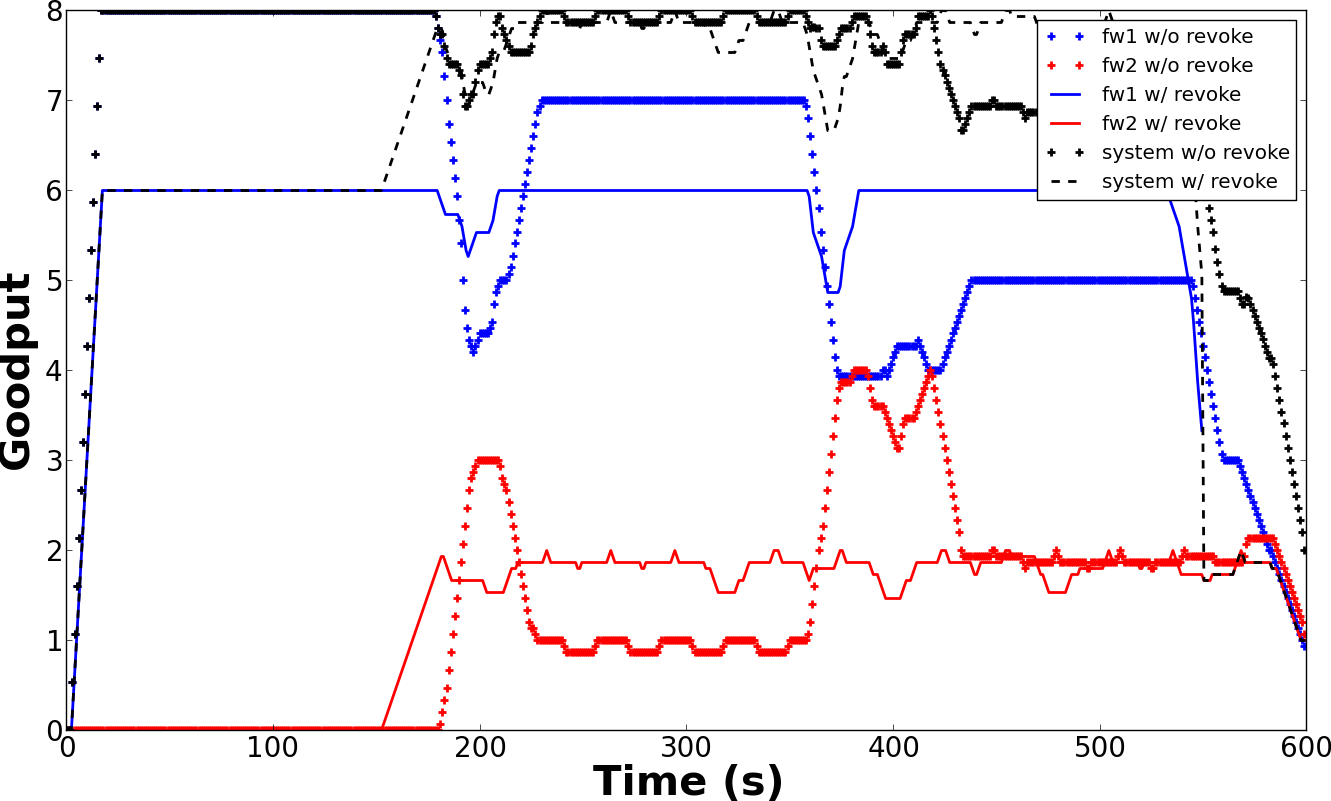
\includegraphics[width=\textwidth]{../results/150_goodput.png}
    \caption{Goodput Results for Scenario A}
    \label{fig:150-goodput}
  \end{subfigure}%
  \hfill
  \begin{subfigure}[t]{0.475\tw}\centering
    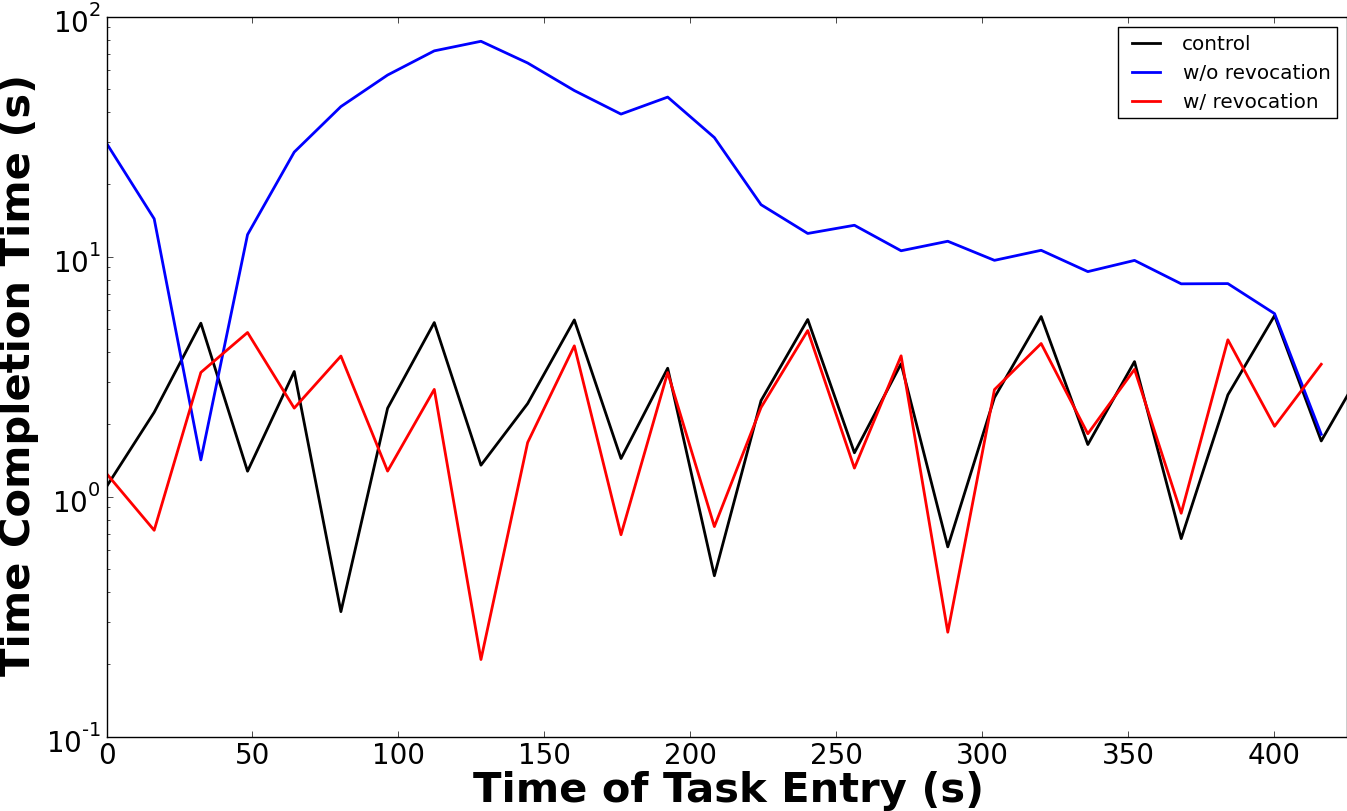
\includegraphics[width=\textwidth]{../results/150_fw_latency.png}
    \caption{Latency Results for Scenario A}
    \label{fig:150-latency}
  \end{subfigure}%

  \caption{\textbf{Goodput and Latency Results for Scenario A}
  Figure~\ref{fig:150-goodput} shows that
  there is significant goodput loss at the beginning due to the fact that tasks that have been running
  for 150 seconds are killed. However, this drastically improves the latency of the second figure as
  seen in Figure~\ref{fig:150-latency}. Without resource revocation, the second framework would have
  latency numbers an order of magnitude larger than in the control. With revocation, the second
  framework's latency numbers matches closely with the control's.}
  \label{fig:150-goodput-latency}
\end{figure*}
